\documentclass[letterpaper,12pt]{article}
\usepackage{fullpage}
\usepackage{courier}
\usepackage[margin=0.75in]{geometry}
\usepackage{listings}
\usepackage{color}
\usepackage{graphicx}
\usepackage[width=6in]{caption}
\usepackage{hyphenat}
\usepackage{multicol}

% define extra colors
\definecolor{dkgreen}{rgb}{0,0.6,0}
\definecolor{purple}{RGB}{159,0,197}

\newcommand*\unparagraph{%
	\par
	\nopagebreak
	\vskip3.25ex plus1ex minus.2ex
	\noindent
}

\lstset{
	language=C++,
	basicstyle=\ttfamily,
	backgroundcolor=\color{white},
	showspaces=false,
	showstringspaces=false,
	frame=none,
	tabsize=3,
	keywordstyle=\color{purple},
	commentstyle=\color{dkgreen},
	stringstyle=\color{blue},
	escapeinside={\%*}{*)}
}

\title{\Large CS 1428\\Quiz 3 Sections L19 and L06} 
\author{Jared Wallace}
\date{}

\begin{document}

\maketitle

\section*{Questions}
\begin{enumerate}
	\item State the discerning difference between for and while type loops:
		\vspace{20mm}
	\item What type of loop might I use for input validation?
		\vspace{20mm}
	\item Write a loop that asks the user for 10 integer values (not looking for input validation here):
		\vspace{20mm}
	\item How many times is a do while loop guaranteed to execute?
		\vspace{20mm}
	\newpage
	\item What is the output of the following code:
	\begin{lstlisting}
for(int i=0; i < 5; i++)
	for(int j = 0; j < 10; j+=2)
	cout << i;
	\end{lstlisting}

\begin{multicols}{2}
	\begin{enumerate}
		\item
			\begin{lstlisting}
11111
22222
33333
44444
55555
			\end{lstlisting}
		\item
			\begin{lstlisting}
02468
02468
02468
02468
02468
			\end{lstlisting}
		\item
			\begin{lstlisting}
12345
12345
12345
12345
12345
			\end{lstlisting}
		\item
			\begin{lstlisting}
12345
123
1
			\end{lstlisting}
		\end{enumerate}
	\end{multicols}
	
\end{enumerate}

\vspace{20mm}

\begin{figure}[ht!]
	\centering
	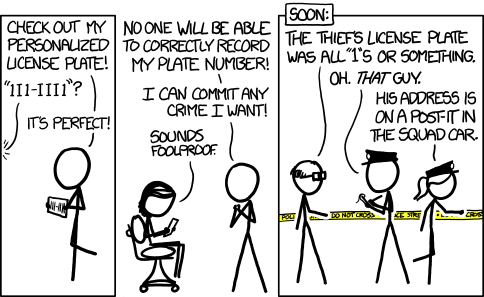
\includegraphics[width=5in]{license_plate.png}
\end{figure}

\end{document}
